\chapter{Methods}\label{chapter:methods}

This chapter describes implementation of the mobile Augmented Reality (AR) pipeline of avatars rendering, and experiments on increasing the DNN's \cite{dnn:stylepeople21} images quality for AR scenario. Section \ref{methods:dev-setup} lists target hardware and software, including the used libraries, tools, and configuration of the baseline model. Section \ref{methods:app} describes the mobile pipeline and algorithmic tricks used to achieve real-time performance. Section \ref{methods:zooms} presents motivation and implementation details for experiments with the DNN's training procedure.

\section{Experimental setup}\label{methods:dev-setup}

The baseline \cite{dnn:stylepeople21} model can be trained on a monocular video sequence of frames with a single person shown from multiple sides.  The training process is carried out on desktop hardware (1 GPU). It takes about 16 hours to complete a single experiment of 500 epochs on about 500 frames, with batch size 8 and generated images with resolution $512 \times 512$ pixels. All training computations are carried out in full-float FP32 numbers format.

There are multiple pre-made training video sequences for the experimentation. They were captured on a stationary monocular smartphone camera. Then for each frame a segmentation mask was predicted using an external pretrained segmentation model Graphonomy \cite{dnn:graphonomy19}, to isolate the person's body from background objects. Next, SMPL-X \cite{dnn:smplx19} body model was fit to all the frames, i.e. there are predicted pose vector $\theta$, body shape vector $\beta$, facial expression vector $\psi$ from which a posed body mesh can be obtained. A few frames were then filtered out from the training set if body fits were misaligned with the source image. It was observed, that the quality of body model fits is critical for the avatars final quality. Hence for the frame of this thesis, the training pipeline adjustments discussed in Section \ref{methods:zooms} will be compared quantitatively and qualitatively only with respect to a training video sequence with the best body model fits at our disposal. A few promising experiments will be repeated with a few other training sequences to verify stability of results. 

For the rest of this report, we will refer to the aforementioned video sequence and its pre-processed data as the \textit{training sequence}. It contains \alert{451} training sample, and a validation set of 13 consequent frames, that do not resemble any other training data. As for a test set, a sequence of difficult premade poses and camera angles was prepared. It includes an animation of extensive gesturing, a view on the avatar from top and bottom, from far away, and close-up to the face. Such poses intend to verify, that the DNN is capable of rendering frames that hardly resemble the training data, yet may be encountered by a user in an AR session.

The baseline DNN \cite{dnn:stylepeople21} detail we start off from, has the following configuration. (spectral ntex prior, multiscale texture, losses and metrics)

Android application target hardware and software
The mobile application is being developed in Java and Kotlin programming languages, only for Qualcomm Snapdragon Soc and Android operating system. Although a variety of devices types fit these criterions, e.g. AR glasses or some VR devices, the application was only tested on latest Samsung smartphones. The main development libraries are: Java Software Development Kit (SDK) and Android SDK.

Libraries used opengl arcore onnx snpe, quantization

Performance of the DNN inference on mobile is measured directly in the application, where a single frame processing is reported step by step via logs. There are measured: time of SMPL-X body mesh inference from a pose vector, time of rendering the DNN's input frame on GPU, time of delay between obtaining this data and receiving it by the DNN, time of DNN's inference, time of output rendering on the screen. In order to measure overheating, a separate application mode is used, where the network is being inferred continuously for a few minutes with a constant random tensor of data. Thus, the computing device is 100\% busy, we use it as an upper bound of power consumption by the device. After the run session if finished, the temperature increase is reported, as well as average latency inference to verify sustainability of high performance. To understand the pipeline performance better, Qualcomm Snapdragon Profiler utility is used, to visualize occupation of computing devices over time, and to reason about potential bottlenecks.

Qualitative assessment of the discussed training pipeline adjustments, is done using a test sequence of body poses, that are hand crafted, and present the avatar from angles that could be potentially observed in AR, e.g. top-down, bottom-up views, strong zoom-in and zoom-out, unseen poses involving rapid hands movements. Each experiment generates a test video from this test sequence. It allows to detect visual artifacts in action, such as flickering, clothes shaking, color defects, blurriness. Since it is hard to reason present and compare these videos within the paper report, a selection of static frames of training, validation and test sequences with the hardest poses are added to the Appending \alert{APPENNDIX}. As already mentioned, in the absence of an absolute metric of visual quality, the visual inspection is the main tool of qualitative assessment in this research. Plots of validation metrics are also examined, but their improvements were frequently found to correlate with the visual quality degradation.


AR experience is being accomplished using ARCore SDK for continuous tracking of real world objects relative to phone's camera. The tracking information is sufficient to draw arbitrary images at respective screen locations. The drawing itself is done directly on GPU by issuing commands of OpenGL application programming interface (API).

The DNN models are to be developed in Python programming language, specifically PyTorch framework for development of DNNs. Such models require a special conversion in order to run them on mobile processors.  Mobile devices with Qualcomm Snapdragon processors require DNN models in Snapdragon Neural Processing Engine (SNPE) format. The whole conversion can be described as follows:
\begin{enumerate}
	\item  PyTorch model is converted to Open Neural Network Exchange (ONNX) format . For it the Python code is run once on example data, in order to record sizes and shapes of all the data flowing through DNN. 
	\item The model in ONNX format is converted to SNPE format, using SNPE SDK. 
	\item The underlying weights of the DNN layers are quantized, from 32-bit floating point numbers to 8-bit integer number format. All input data has to be quantized as well.
\end{enumerate}

The intermediate conversion to ONNX format is required due to absence of software for direct conversion from PyTorch models to SNPE. The quantization is a preferable option, because it allows computing the DNN on modern DSP, NPU accelerated devices.

Preparation of an input tensor for the DNN is a trivially parallel task. In essence, it is a rendering of a human mesh with a multichannel texture. It is suitable for execution on GPU and can be done using OpenGL API or OpenCL API.

Spectral coordinates \cite{aux:spectral10}.

\section{Mobile application development}
\label{methods:app}
\begin{figure}
	\centering
	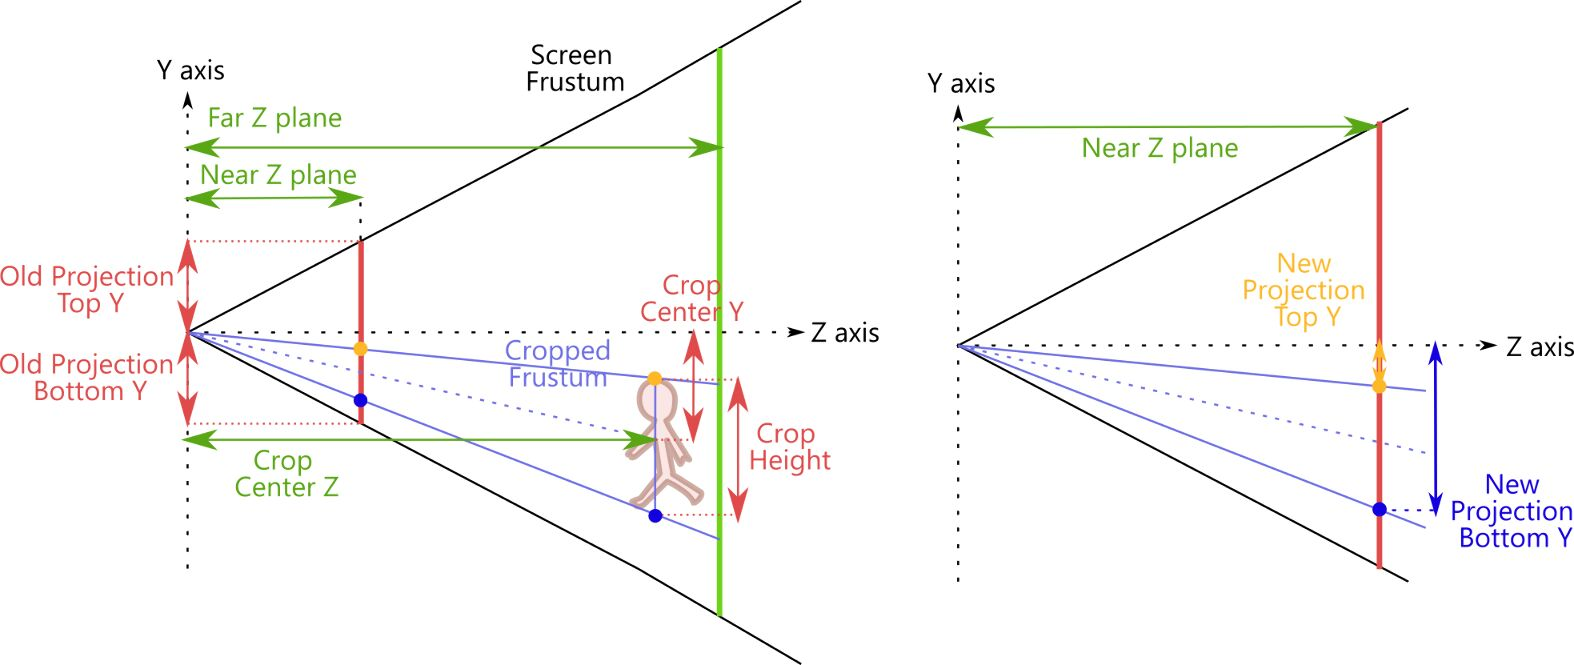
\includegraphics[width=\textwidth]{\imgfp/dynamic_crop/dynamic_crop}
	\caption{A 3D space with origin at the camera, and axes aligned with camera directions ($x$ - right, $y$ - top, $z$ - front). The figure shows a slice of this space with $x=0$, illustrating the dynamic projection crop. \textit{(Left)} The near plane of the old screen frustum is defined by a $z$ distance (arbitrary), and $x$/$y$ coordinates of the frustum borders (top/bottom coordinates on illustration). \textit{(Right)} To make the projection cropped around the avatar body, we compute an axis-aligned bounding box of the body, then project its spans onto the near plane, obtaining top/bottom borders, defined by intersection coordinates of the projection lines and the old near plane. The new frustum will have the same near and far planes as the old one, to ensure preservation of perspective.}
	\label{fig:dynamic_crop_math}
\end{figure}

%TODO
\alert{TODO: Explain in details}
\begin{itemize}
	\item SMPL-X inference on mobile
	\begin{itemize}
		\item  "ON CPU" -- Pre-inference of shape blendshapes into a default posed mesh, load as a GPU buffer into OpenGL
		\item "ON CPU" -- Pre-compute indices of 12 the most influential joints for every mesh vertex, pre-load them on GPU as well.
		\item "ON CPU" -- On each frame compute posed joints (i.e. 55 rotation matrices): unwrap 3 axis angles into matrices following Rodrigues formula for rotations, multiply matrices in topological order to combine rotations of multiple joints. Load the matrices on GPU as shader uniforms (shared by all vertices)
		\item "ON GPU Vertex Shader" -- find a weighted sum of rotation matrices for each vertex (only 12 matrices to add up, using the most influential joints indices, without it 55 matrices would need to be added per each vertex). Project each vertex onto image, using a combination of extrinsic and intrinsic matrices of the camera.
	\end{itemize}
	\item Rasterization with a neural texture and quantization overcoming OpenGL limitations
	\begin{itemize}
		\item OpenGL can only render images with 4 channels RGBA. If rendering 16 channels naively, it requires to render 4 images with 4 channels, then send them to the DNN, and permute channels from 4xHxWx4 to 1xHxWx16, which is long to do on each frame (takes up to 20 ms)
		\item Using quantization, we can let network accept each channels as an 8-bit integer number. Then in OpenGL we can quantize in parallel rasterized pixels from 4-byte floats to 1-byte integers, pack them together with 4 neural channels per OpenGL channel, and then we do not need to permute channels, the input goes straight into the DNN and the first convolution starts immediately. The visual quality loss is not drastic
		\item Using quantized numbers, it also opens an opportunity to run on Digital Signal Processor (DSP), which is designed to do fast quantized computations (mainly because of bit-fiddling shortcuts possible with integers, and not with IEEE floating point numbers). Overall the performance is more than real-time with up to 640 px resolution
	\end{itemize}
	\item Dynamic camera frustum cropping
		\begin{itemize}
			\item Around view span -- On every frame compute coordinates of joints in camera space, find a XY-bounding box for them. Project bounds of this box onto the image, and find adjustments of top-bottom-left-right-near-far parameters of the camera frustum. Calculate a new projection matrix to fit only the bounding box of the avatar. Rasterize an input frame with this matrix. Infer the network and place the output using offset computed from the updated projection matrix
			\item Auto-zoom to reducing frame waste -- detect if bounding box of joints is cut off by the mobile screen. Zoom in the projection matrix to the avatar to compensate cut off parts. This will allow to see the avatar parts rendered in bigger resolution (thus DNN has to be trained on zoom scale too)
		\end{itemize}
	
	\item \alert{TODO: parallelization}
\end{itemize}
%\begin{figure}[!htbp]
%	\centering
%	\begin{lstlisting}[
%		language=C++,
%		numbers=none,
%		basicstyle=\ttfamily,
%		keywordstyle=\color{NavyBlue}\textbf,
%		frame=single,
%		extendedchars=true,
%		tabsize=4,
%		morekeywords={interface, string},
%		]
%public interface IVisualizer
%{
%	string GetDescription();
%	void VisualizeModel(Stream model, ModelMetaBase modelMeta, 
%	Stream materialLibrary, Stream[] materialFiles);
%	void Shutdown();
%} 
%	\end{lstlisting}
%	%	\captionsetup{justification=centering}
%	\caption{Blah blah example}\label{res:code:example}
%\end{figure}

\section{Improving quality of synthesized images}\label{methods:zooms}
\begin{figure}
	\centering
	\begin{subfigure}[b]{0.48\textwidth}
		\centering
		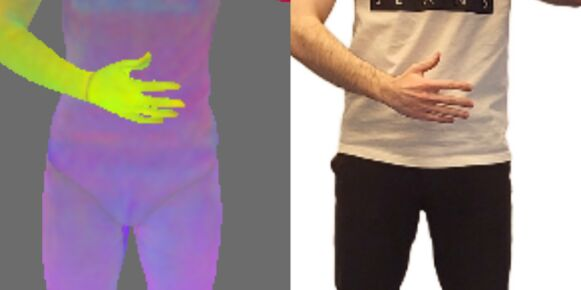
\includegraphics[width=\textwidth]{\imgfp/cam_augs/img}%
		\caption{}
		\label{fig:cam_aug:before}
	\end{subfigure}
	\begin{subfigure}[b]{0.48\textwidth}
		\centering
		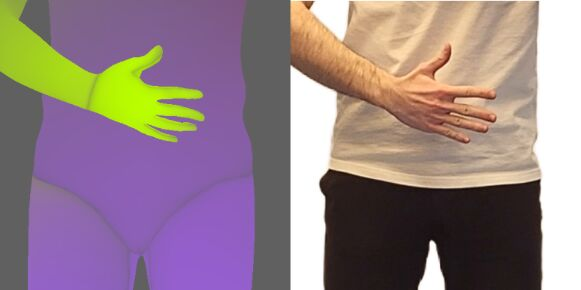
\includegraphics[width=\textwidth]{\imgfp/cam_augs/cam}%
		\caption{}
		\label{fig:cam_aug:after}
	\end{subfigure}
	\caption{(\protect\subref{fig:cam_aug:before}) Implementation of zooming using image-space augmentations. The body mesh is rasterized in full-body, the ground truth is transformed once to be in an alignment with the rasterization. Then both are magnified, loosing a lot of quality. (\protect\subref{fig:cam_aug:after}) Using camera-space augmentations, the virtual camera used for rasterization replicates zooming by moving towards the avatar. The input image can be made arbitrarily sharp. The ground truth image is still transformed with image-space augmentations, but only once, preserving a bit of quality. }
	\label{fig:cam_aug}
\end{figure}

The baseline DNN architecture \cite{dnn:stylepeople21} proved to be sufficient to render FB images of avatars. However, we found out that the rendering network cannot reliably render parts on the body that were never seen during training, most commonly under boots surface, and top of the head. At best, these places can be rendered as random patches of color, e.g. from clothes or skin. Intuitively it is so, because in these areas the neural texture will contain default values during the whole training process. If the renderer learns quickly enough to map such default values to skin or clothes, the chance is that the texture overall will not move much away from the defaults. Although the unseen parts are not rendered correctly from reconstruction point of view, it does not hurt overall accuracy. On the other hand, there is a chance that the neural texture will significantly move away from the default initialization. Thus, after many epochs the default values contained in the unseen parts will be outliers that the renderer does not expect to see. This may trigger it to render abnormal color or fail segmentation prediction. Attempts on dealing with this artifact will be given shortly after.

Besides the unseen parts, after launching the model
\alert{TODO: Motivation and pre-conclusions}

Researched adjustments:
\begin{itemize}
	\item Camera space affine augmentations module (for Python) to eliminate need of augmenting prerasterized frame (which will lead to quality loss on strong zooms)
	\item Zooming to different joints (or mesh vertices) with different scale range 
	\item Regularization of Batch Normalization layers to prevent overfit (and Spurious Correlations as result): collecting statistics on FB scale only, or on zoom scale only; using current statistics to train or not
	\item Accumulating gradients for more than 1 batch before making optimization step
	\item Adam Optimizer without 1st momentum in neural renderer, discriminator
	\item Fine tuning a zoom-trained model on FB to restore FB quality and to preserve neural texture high frequency details
	\item Other normalization layers: Instance norms, Group norms, No norms
	\item Adam optimizer of the neural texture - do not decay momentum of pixels with 0 analytic gradient (unseen in the current batch)
	\item Capacity of neural texture, encoder, decoder
	\item Gradient norm clipping
	\item Learning rate scheduling with warmup and later annealing
	\item Concatenate input neural image to deeper activations of the encoder
	\item More strong affine augmentations 
	\item Batch normalization without learned affine parameters, or without tracking running statistics 
	\item Single-scale neural texture, compared to multiscale-texture
	\item Homogeneous augmentations in a single optimization batch (to prevent mixing of statistics)
	\item Disabling GAN losses
	\item Initializing neural texture training from a stable pretrained checkpoint, or random noize, compared to spectral initialization
	\item Disable discriminator on zooms, or disable discriminator on FB
	\item Equal loss weights
	\item Using scale probability distribution to prioritize FB scale and show close-up and far-out ever so rarely
	\item Dropout2d to nullify random feature maps after convolutions: in encoder, in decoder, in both
	\item Change input rasterization background to not 0 (which is a valid value on the neural texture), but to ntex.abs()*2
	\item Add gaussian noize to input rasterization, or neural texture, or ground truth
	
\end{itemize}